\documentclass{beamer}

\providecommand{\rootdir}{../doc}

% \def\privateData{private_data}

% % % % % % % % % % % % % % % % % % % % % % % % % % % % % % % % % % % % % % % %

\usepackage[english]{babel}
\usepackage{ifthen}
\usepackage{color}
\usepackage{hhline}
\usepackage{adjustbox}
\usepackage{amsmath,amsfonts, amssymb}
\usepackage{mdframed}
\usepackage{relsize}

\usepackage{tikz, skak}
\usetikzlibrary{fit, matrix, positioning, shapes, decorations.pathreplacing,
                shapes.geometric, chains, arrows, calc }




\newcommand{\red}[1]{{\color{red} #1}}
\newcommand{\green}[1]{{\color{green!50!black} #1}}
\newcommand{\orange}[1]{{\color{orange} #1}}
\newcommand{\blue}[1]{{\color{blue} #1}}

\newcommand{\blap}[2][0pt]{\vbox to #1{\hbox{#2}\vss}}


\newcommand{\resizeinput}[2][1]{%
  \resizebox{#1\textwidth}{!}{\input{#2}}%
}

% % % % % % % % % % % % % % % % % % % % % % % % % % % % % % % % % % % % % % % %
% from MathDefs.tex

\def\Re{\mathbb{R}}

\def\behaviour{\mathrm{behaviour}}
\def\act{\mathrm{act}}
\def\react{\mathrm{react}}
\def\state{\mathrm{state}}
\def\action{\mathrm{action}}
\def\msg{\mathrm{message}}

\def\coh{\mathrm{coh}}
\def\rel{\mathrm{rel}}
\def\fold{\mathit{fold}\,}

\def\Bool{\mathrm{Bool}}
\def\Candidate{\mathit{Candidate}}
\def\Details{\mathit{Details}}
% \def\Context{\mathit{Context}}


\providecommand{\letIn}[2]{
  \begin{aligned}[t]%
    & \mathit{let}\, #1 \\%
    & \mathit{in}~ #2%
  \end{aligned}%
}


% % % % % % % % % % % % % % % % % % % % % % % % % % % % % % % % % % % % % % % %

% https://tex.stackexchange.com/questions/45938/error-when-using-colour-in-author
\ifthenelse{\isundefined{\privateData}}
           {\author{\texorpdfstring{\color{red} Anonymous}{???}}}
           {\input{\privateData}}

% % % % % % % % % % % % % % % % % % % % % % % % % % % % % % % % % % % % % % % %

\title{University class schedule generation using personalizable agents negotiation}
\subtitle{Thesis for Master of Science in Intelligent Systems}
\institute[ITESM]{Tecnol\'{o}gico de Monterrey}
\logo{\includegraphics{../doc/escudo-itesm}}
\date{May, 2017}

% % % % % % % % % % % % % % % % % % % % % % % % % % % % % % % % % % % % % % % %


\mode<presentation>

\begin{document}

\frame{\titlepage}

% % % % % % % % % % % % % % % % % % % % % % % % % % % % % % % % % % % % % % % %
% \input{1-UCSP}
% \documentclass[ThesisDoc]{subfiles}

\providecommand{\rootdir}{.}

\def\Re{\mathbb{R}}

\def\domain{\mathrm{domain}}

\def\domain{\mathrm{domain}}
\def\pop{\mathrm{pop}}

\def\behaviour{\mathrm{behaviour}}
\def\act{\mathrm{act}}
\def\react{\mathrm{react}}
\def\state{\mathrm{state}}
\def\action{\mathrm{action}}
\def\msg{\mathrm{message}}

\def\coh{\mathrm{coh}}
\def\cohi{\mathrm{\widetilde{coh}}}
\def\rel{\mathrm{rel}}
\def\fold{\mathit{fold}\,}

\def\restrC{\accentset{C}{\xi}}
\def\restrT{\accentset{T}{\xi}}
\def\restrS{\accentset{S}{\xi}^p_i}
\def\restrW{\accentset{W}{\xi}^p_i}

\def\ctx{\mathit{ctx}}
\def\codom{\mathrm{codomain}}
\def\maybe{\mathrm{Maybe\,}}

\def\TRUE{\mathit{TRUE}}


\begin{document}

% \green{Explicar que son los CSP}
\chapter{Constraint Satisfaction Problems}
\label{chapter:csp}

% \green{Poner una definición no formal}
% \medskip

There are many problems that require positioning or assigning something,
respecting established \emph{restrictions}. \emph{Graph coloring} and
\emph{n-queen} chess problem are classical constraint satisfaction problems (CSPs).

% \medskip
% \green{Poner algunos ejemplos}
% \medskip

The graph coloring problem comes from cartography, where it was needed to color
countries on political maps, in such a way that no country had a land border with
a country of the same color. It was found that \textbf{any} map can be colored
with only four colors.

The n-queen problem is known in chess as \emph{eight queen puzzle}.
Queens in chess can move/attack to/at any square,
that is in a the same row, column or diagonal with the queen.
In the puzzle one needs to place eight (the size of a chess desk)
queens on the desk, so that none of them is threatened by another.
N-queens problems is a generalization of that puzzle, where $n$ queens need
to be placed on a $n \times n$ desk.

Constraint satisfaction problems are found in many areas:
machine vision, natural language processing, theorem proving,
planning and in our problem --- scheduling \cite{MAS}.


\section{Formal definition}
%%%%%%%%%%%%%%%%%%%%%%%%%%%%%%%%%%%%%%%%%%%%%%%%%%%%%%%%%%%%%%%%%%%%%%%%%%%%%%%%
\noindent
Formally speaking, a CSP is defined by its \emph{variables} $V$ with the
corresponding \emph{domains} and the \emph{constraints} $\{\xi\}$
over values assignation \cite{MAS}.

\begin{align*}
  V                &= \{v_i\}_{i=1}^N
& \{{\dot v}^i_j\} &= \domain(v_i)
& \xi              &: \{{\dot v}^i_\ast\}_{i=1}^N \mapsto [0,1]
\end{align*}


A variable defines a ``slot'' that can hold a value from the corresponding domain.
A solution to CSP is an assignation of the values ${\dot v}^i_\ast$
to the variables $V$, such that all the restriction hold.
\begin{equation}
  {\dot V} = \{{\dot v}^i_\ast\}_{i=1}^N \text{is a solution}
   \iff \forall \xi \in \{\xi\} \Rightarrow \xi({\dot V}) = 1
\end{equation}

The constraints above are defined in the most generalized form,
over the entire solution. There is a particular case, that is found in many problems
--- \emph{binary constraints}, imposed on \emph{pairs} of values:
$$\xi_2 : \left< {\dot v}^i_\ast, {\dot v}^j_\ast \right> \mapsto \{0,1\}$$

If all constrains are binary, than the satisfaction condition is
$$\forall \xi_2     \in \{\xi\},~
  \forall v_i, v_j  \in V | v_i \not= v_j
~ \Rightarrow ~ \xi_2(v_i, v_j) = 1
$$

\medskip

In the graph coloring problem, the variables are the \emph{colors to be assigned}
for each graph node $\{n_i\}_{i=1}^N$. In this case, all the variables have
the same domain values: four colors, for example \textit{Red}, \textit{Green},
\textit{Blue} and \textit{Yellow}. The constraint is binary and depends on graph
structure:
$$ \xi_2(x,y)= \begin{cases}
  0 & \mbox{if } \exists \text{~edge~} x \leftrightarrow y
                ~\land \text{~color~} x = \text{color~} y \\
  1 & \text{otherwise}
\end{cases}
$$

% For the n-queens problem, there are two ways of representing the variables.One
% can see queens' positions as a single variable --- pairs $\left< x,y \right>$.
% But it's better to handle them separately, as it would be shown in \ref{TODO}.
% In this case each queen would have two variables:
% horizontal and vertical positions $x$ and $y$.

For the n-queens problem, the variables are queens' positions ---
pairs $\left< x,y \right>$, where $x$ is queen's horizontal position and
$y$ is the vertical one. The restrictions can be gathered within a single
constraint function:
$$\xi_2(\left<x_1,y_1\right>, \left<x_2,y_2\right>) =
    \begin{cases}
      0 & \mbox{if } \begin{cases}
                        &      x_1 = x_2  \lor y_1 = y_2 \\
                        \lor~& x_1 = y_2 \land x_2 = y_1 \\
                        \lor~& x_1-y_1 = x_2-y_2\\
                        \lor~& x_1+y_1 = x_2+y_2
                     \end{cases} \\
     1 & \text{otherwise}
    \end{cases}
$$

\begin{figure}
  \begin{subfigure}[b]{0.3\textwidth}
    \centering
  	\subfile{\rootdir/img/NQueens/Restrictions.tikz}
  	\caption{Queen moves/attacks.}
  	\label{fig:QueenMoves}
  \end{subfigure}
  \hfill
  \begin{subfigure}[b]{0.3\textwidth}
    \centering
  	\includegraphics[trim=100 260 370 370, clip] % width=\textwidth
               {\rootdir/img/easteuro}
  	\caption{Part of Central Europe \cite{UN-CEU-Map}.}
  	\label{}
  \end{subfigure}
  \hfill
  \begin{subfigure}[b]{0.3\textwidth}
  	\centering
    \subfile{\rootdir/img/ColorMap/CEUMapGraph.tikz}
  	\caption{Graph coloring problem.}
  	\label{fig:ColoringGraph}
  \end{subfigure}
  \caption{CSP examples}
\end{figure}

  In our \emph{university classes scheduling} problem (UCSP) the variables
are personal schedules, called \emph{timetables} in this thesis,
for each \emph{participant}: professor and group/student.
  A timetable consists of the day-time slots, where classes can be put.
  A \emph{class} is formed for teaching a group a specific \emph{subject},
connecting the participants (of each kind) and establishing a classroom and
the beginning--end \emph{time}.
  Problem \emph{constraints} can be divided into:
\begin{enumerate}
  \item \underline{Class constraints}: a class should be a productive event, so
    a professor should be able to \emph{teach} the class, the classroom should
    have the \emph{capacity} to hold all the students and be properly \emph{equipped},
    and the group should be \emph{enrolled} to class subject
    (further called \emph{discipline}).
  \item \underline{Time constraints}: no participant can have two classes
    at the same time (or intersecting in time), as mentioned before.
  \item \underline{Strong restrictions}: the restrictions, put on a participant, that
    \emph{must} be respected. May include working hours, fixed lunch recess time,
    and any other institution or person specific \emph{obligations}.
  % \item \red{\underline{Weak restrictions} (MOVE)}: the restrictions, that \emph{should} be respected,
  %   but are not critical to the solution. Compliance with these restrictions
  %   raises \emph{solution quality}, but it is assumed that the all of them
  %   cannot be fully met for all the participants --- they are intended to
  %   represent personal \emph{preferences}.
\end{enumerate}

\bigskip

%%%%%%%%%%%%%%%%%%%%%%%%%%%%%%%%%%%%%%%%%%%%%%%%%%%%%%%%%%%%%%%%%%%%%%%%%%%%%%%%
  Until now we were speaking about restrictions satisfaction, but the problem can
be extended to an \emph{optimization} one by defining an
\emph{objective function} over the values configurations.

  Unlike the restrictions (that yield boolean result), the objective functions
should have continuous codomains:
$$\tilde\xi : \{{\dot v}^i_\ast\}_{i=1}^N \mapsto \Re$$
  In order to facilitate the calculations and erase the internal differences of
the objectives, it's often required that the functions must be normalized:
the co-domains are restricted to $[-1,1]$ or $[0,1]$ intervals.

  For example, in case of our UCSP,
one can add \underline{personal preferences} or some institution criteria as
optimization parameters.
  Compliance with the preferences raises \emph{solution quality},
but it is assumed that the all of them cannot be fully met for all the
participants, because \emph{personal} preferences are often
contradictory for different persons.

\section{Solution Methods}
%%%%%%%%%%%%%%%%%%%%%%%%%%%%%%%%%%%%%%%%%%%%%%%%%%%%%%%%%%%%%%%%%%%%%%%%%%%%%%%%
% \green{Explicar por qué son importantes computacionalmente}\\
% \medskip

% \noindent
  Solving these problems usually presents difficulties due to the amount of
possible combinations to consider for a solution. Let's have a look at
some university schedule.
  For example, six working days in a week and twelve time slots every day
(every hour from 8:00 to 20:00), would yield $6 \times 12 = 72$ options
to place each class.
  Given that each group needs, for example, five different disciplines to be assigned,
there would be $\multibinom{72}{5} = \num[group-separator={,}]{18474840}$
possible classes assignments for each group,
even without considering professors and classrooms.

% \bigskip
% %%%%%%%%%%%%%%%%%%%%%%%%%%%%%%%%%%%%%%%%%%%%%%%%%%%%%%%%%%%%%%%%%%%%%%%%%%%%%%%%
% \green{Explicar formas de resolver los CSP} \todo
\medskip
\noindent

  The researchers have been looking for means of solving such
problems within reasonable time.
  During the last years different algorithms and techniques where developed,
such as
\emph{dynamic constraint satisfaction based on extension particle swarm
      optimization algorithm} \cite{CSPswarm},
\emph{dynamic state bounding} \cite{CSPdynStateBound},
\emph{conflict-vector detection} \cite{CSPtimetable},
\emph{neural networks} \cite{CSPneuro},
\emph{ant colony optimization} \cite{CSPcunningACO, CSPlimmemACO},
\emph{selective hyper-heuristics} \cite{CSPhypHeur},
\emph{quantum-inspired genetic algorithm} \cite{QuantumGeneticAlgorithm}
and \emph{agents} \cite{CSPagent2013, CSPagent2014, DCSPagent1998}.

\medskip

Those methods do not seek for the optimal solutions, focusing instead on
``rather good'' ones, that can be obtained within reasonable time using admissible
computing resources.

\bigskip

\noindent
Some agent solution methods are presented in section \ref{sec:CSP-Agents}.

% % % % % % % % % % % % % % % % % % % % % % % % % % % % % % % % % % % % % % % %
\subsection{Genetic Algorithm}
GA is an evolutionary computational method for solving optimization problems,
including constraints satisfaction. The method is inspired by \emph{evolution
theory}, its genetic part to be concrete. It is known that living organisms
store information about themselves and transmit (part of) it to its offspring.
In case of sexual reproduction, each participating sex gives its share of
genetic information, thus ``mixing'' parents properties in the offspring.
It's called \emph{crossover}.
Crossover can create combinations of the parents, but not create something new.
The latter is provided by \emph{mutations} --- random changes in the genome, due
to copying errors. Because of mutation's randomness, the results cannot be known
in advance, and such event might both better or worsen the ``victim''. Mutations
are relatively rare in the nature, thus maintaining species populations more or
less alike.

But if the mutations are rare, then how are the new properties fixed within
populations? The response to this isn't found in the genetics, but rather in
organism's \emph{adaptation} to the environment. A property that gives an
\emph{advantage} before the rest of the population
\begin{enumerate*}[1)]
  \item raises organism's chances of survival, extending mean life length and
        potential number of children within its lifetime;
  \item raises organism's ``value'' in the eyes of potential mate, thus further
        increasing potential size of its offspring.
\end{enumerate*}
With time, the property is spread throughout the population, because of the
advantages it gives.

\bigskip\noindent
Genetic algorithms search for better \emph{adopted} ``organisms'', described
by their genetic code --- chromosomes, using \emph{crossover} and \emph{mutations}
as its \emph{genetic operations}.
The chromosomes are \underline{lists of \emph{genes}} --- variables with finite
domains. The degree of \emph{adaptation} is calculated by
\underline{\emph{fitness function}}.

GAs are iterative algorithms, working with \emph{populations}, that consist of
\emph{chromosomes}, representing possible solutions. The algorithms search
for better \emph{fitted} solutions, trying to maximize mean population
\emph{fitness} on each iteration.
Notable advantage of genetic algorithms is that they are capable of
``getting out'' \underline{local} maximums due to the mutations, thus finding
the \underline{global} maximum, provided adequate configuration.

\begin{enumerate}[start=0]
  \item Create initial population (randomly).
  \item\label{list:GA:start} Evaluate \emph{fitness} of each chromosome in the population.
  \item If \emph{stop criterion} applies, return best chromosomes and terminate.
  \item\label{list:GA:xover} Select best chromosomes and apply \emph{crossover}.
  \item\label{list:GA:mutate} Select chromosomes for mutation and \emph{mutate} them.
  \item Create new population from the crossover children (\ref{list:GA:xover}),
        mutated chromosomes (\ref{list:GA:mutate}) and the original population
        (\ref{list:GA:start}).
        Go to \ref{list:GA:start}.
\end{enumerate}

\subsection{Quantum-inspired Genetic Algorithm}
An interesting modification of Genetic Algorithm (GA), based on the concept and
principles of \emph{quantum computing} --- QGA, was proposed in article
\cite{QuantumGeneticAlgorithm}.
Instead of being represented by a list of \emph{genes}, as in classical GAs,
in QGA a chromosome is represented by a \emph{Q-bit individual}.

\emph{Q-bit} is the quantum counterpart of the classic bit --- the smallest
unit of information. While a normal \emph{bit} can take either 0 or 1 values,
a \emph{Q-bit} can take any \emph{superposition} of the tho states, including
margin values: states 0 and 1. The main difference is that such ``bit'' can be
0 and 1 at the same time, just like famous Schrodinger's cat, that is both dead
and alive. The state of a Q-bit can be represented by two complex numbers
$\alpha$ and $\beta$, that denote the probabilities of a Q-bit being found in
states 0 and 1 respectively.
The values must be normalized: $|\alpha|^2 + |\beta|^2 = 1$.

A \emph{Q-bit individual} of $m$ Q-bits is defined as
\begin{equation}
\left[
  \begin{array}{cccc}
  \alpha_1 & \alpha_2 & \dots & \alpha_m \\
  \beta_1  & \beta_2  & \dots & \beta_m  \\
  \end{array}
\right]
\end{equation}

One of the practical advantages, claimed my the article, is:
\begin{displayquote}
  Evolutionary computing with Q­-bit representation has a better characteristic
  of population diversity than other representations, since it can represent
  linear superposition of states probabilistically.
\end{displayquote}
It presents an example of a three-Q-bit individual, and shows its equivalence
to 8 classical chromosomes of 3 genes at once.

\medskip\noindent
Major differences are found in the \emph{genetic operators} applied:
neither crossover or mutations are used. Instead, tournament selection strategy
with elite retaining model is used to generate new populations.
It works as follows:
\begin{enumerate}
  \item Tournament set --- a set $K$ individuals, is randomly selected from
        the population.
  \item A random number $r$ (between 0 and 1) is selected.
  \item If $r < 0.8$ (empirically established by the authors), then the fittest
        individual in the tournament set is chosen for reproduction.
        Otherwise, any chromosome is chosen from the tournament set.
\end{enumerate}
\noindent
After selecting intermediate population of the same size, \emph{quantum rotation gate}
is applied to each individual's Q-bits, creating new population.
The angle used is selected from a table, provided by the authors.

While not providing explicitly any stop criteria for the proposed algorithm,
the authors have compared their method with classical GA, using same number
of generation as stop criterion in both.
University classes scheduling problem was selected for the tests.
The presented results show better final fitness and faster convergence rate for
the proposed QGA.


\section{Distributed problems}
%%%%%%%%%%%%%%%%%%%%%%%%%%%%%%%%%%%%%%%%%%%%%%%%%%%%%%%%%%%%%%%%%%%%%%%%%%%%%%%%
Agents approach allows solving CSPs in a distributed manner by distributing
the problem knowledge and constraints
\cite{DCSPagent1998, DCSP2013, CSPagent2014, MAS, MAS-Survey}.

\begin{displayquote}[\cite{MAS-Survey}] % \cite[p.~2]{MAS-Survey}
  For example, a constraint satisfaction problem can often be
  decomposed into several not entirely independent
  subproblems that can be solved on different processors. $\dots$
  MAS (Multiagent System) allows the sub-problems of a constraint satisfaction
  problem to be subcontracted to different problem solving agents with their own
  interests and goals.
\end{displayquote}

\noindent
Such problems are \emph{Distributed Constraints Satisfaction Problems} (DCSPs).
\begin{displayquote}[\cite{MAS}] % \cite[p.~4]{MAS}
  In a distributed CSP, each variable is owned by a different agent. The goal is
  still to find a global variable assignment that meets the constraints, but each agent
  decides on the value of his own variable with relative autonomy. While he does
  not have a global view, each agent can communicate with his neighbors in the
  constraint graph.
\end{displayquote}


University class scheduling problem fits into a the DCSP class:
\begin{itemize}
  \item Some constraints are agent-specific: strong restrictions and
        personal preferences.
  \item Classes assignments in form of \emph{candidates} are distributed between
        the negotiating agents (representing groups and professors).
\end{itemize}

The original UCSP is decomposed in a set of sub-problems, represented by some
participants. A sub-problem consist in resolving constraints over an agent's
\emph{candidate}, while considering the \emph{opinions} of \emph{neighboring}
agents.

The sub-problems are then recomposed into a schedule, resolving any conflicts
between the sub-solutions with the established rules.

\end{document}

% % % % % % % % % % % % % % % % % % % % % % % % % % % % % % % % % % % % % % % III
\section{Formal Definition}

\begin{frame}{University Class Scheduling Problem}
  \centering
  \begin{block}{Required Data}
    \begin{columns}[t]
      \begin{column}{.4\textwidth}
        \begin{block}{Disciplines $\{d_i\}$}
          \begin{itemize}
            \item academic program
            \item equipment requirements
          \end{itemize}
        \end{block}
      \end{column}
      \begin{column}{.4\textwidth}
        \begin{block}{Groups $\{g_i\}$}
          \begin{itemize}
            \item disciplines needed
            \item personal constraints
          \end{itemize}
        \end{block}
      \end{column}
    \end{columns}
    \begin{columns}[t]
      \begin{column}{.4\textwidth}
        \begin{block}{Classrooms $\{r_i\}$}
          \begin{itemize}
            \item capacity
            \item equipment
          \end{itemize}
        \end{block}
      \end{column}
      \begin{column}{.4\textwidth}
        \begin{block}{Professors $\{p_i\}$}
          \begin{itemize}
            \item able to teach (disciplines)
            \item personal constraints
          \end{itemize}
        \end{block}
      \end{column}
    \end{columns}
    \begin{columns}
      \begin{column}{.4\textwidth}
        \begin{block}{Working Days $\{\bar{d}_i\}$}\end{block}
      \end{column}
      \begin{column}{.4\textwidth}
        \begin{block}{Discrete Time $\{\bar{t}_i\}$}\end{block}
      \end{column}
    \end{columns}
  \end{block}
\end{frame}

\begin{frame}[label=candidate-def]{University Class Scheduling Problem}
  \begin{block}{Class Core $\mathrm{cc} \sim \left< d, g, p \right>$}
    \emph{possible} class (of discipline $d$) for group $g$,
    taught by professor $p$
  \end{block}
  \begin{block}{Class $ c \sim \left< \mathrm{cc}, r, \bar d, \bar t_b, \bar t_e \right> $}
    \emph{concrete} class, with day, time (beginning \& end) and room
  \end{block}
  \begin{block}{Candidate $\tilde{c}_a=\{c ~|~ c\,\mathrm{mensions}\,a\}$}
    set of \alert{valid} classes, assessed using \underline{coherence},
    proposed by $a$
  \end{block}
  \begin{block}{Schedule $= \bigcup\limits_{\forall\,a}\tilde{c}_a$}
    set of \alert{\underline{all}} proposed classes, assessed by every group and
    professor

  \end{block}
\end{frame}

\frame{
  \trimbox{30pt 0 0 0}{
    \resizeinput{\rootdir/img/ConnectionMatrix/Candidates-content.tikz}
  }
}

% \documentclass[ThesisDoc]{subfiles}
\begin{document}

\providecommand{\rootdir}{.}

\section{Coherence}
\label{sec:Coherence}


% \green{Explicar qué es coherencia.}
% \medskip

In simple worlds, \emph{coherence} is a state or measure of some \emph{pieces}
fitting together into a whole. Coherence can be applied to almost any aspect of
the universe. Stable orbits require coherence between the observed laws of physics
and universal constants, the speeds and masses of the bodies in the system.
A healthy society asks for coherence between the people and their roles within
the system. An organism requires coherence between its organs in order to operate;
its interactions with the environment must be coherent with its necessities and
surrounding conditions. The notion of coherence is very powerful because of its
generality. Based on a proper logic, coherence can be used to judge about systems
and to test different situations or proposals.

\begin{displayquote}
The consistency or \emph{coherence} within a logical or mathematical
system, means that $p$ and $\neg p$ must not be derivable from the
basic assumptions in accordance with the observance of the syntactical
rules \cite{Daya60}.
\end{displayquote}


\subsection{Coherence theory}

\begin{displayquote}
Coherence theory is a psychologically motivated motivational cognitive theory with
foundations in philosophy that approaches problems in terms of the satisfaction
of multiple constraints within networks of highly interconnected elements
\cite[p.~19]{UAB-Thesis}.
\end{displayquote}

Thagard, in his work \cite{Thagard89}, shows how \emph{explanatory coherence}
can be used to test hypothesis against propositions for proving scientific theories
and reasoning about many other situation. He says that a hypothesis coheres
with given propositions if it explains, is explained, offers analogous explanation or
participates in other explanations. The propositions that stand for observations
have a degree of acceptability. Propositions are incoherent if they contradict
each other.

Another interesting usage, given by Thagard, using his \emph{explanatory coherence}
theory for \emph{Adversarial Problem Solving} (APS).
APS consists in understanding of opponent's strategy and anticipation of his actions
with the purpose of successful counteraction and ultimate victory.
These problems are competition ones: it could be war or business strategy,
different games, and any other areas, that involve gaining the upper hand
on adversaries. Thagard states that the judgments, based on the coherence theory,
can be important for inferring the plans of the opponent and deceiving him
\cite{ThagardAPS92}.

\medskip

Later Thagard published that coherence can be understood in terms of maximal satisfaction
of multiple constraints and in this form it can be used to solve problems in
diverse areas, such as logic, mathematics, law, ethics, rationality, etc \cite{ThagVerb98}.

In his theory, the coherence problem is about partitioning a graph of
\emph{information pieces}, interconnected by positive or negative weighted
constraints, that enhance or diminish partition's coherence.
The coherence-maximizing partition is the one that has maximum number of constraints
satisfied.

An example of partitioning by Thagard's method is given in figure \ref{fig:UAB-partition}.
The information graph $\mathcal{V}$ consists of
classes $C_1,\dots,C_4$, also there are three possibilities for
class $C_1$ placement and two for class $C_4$. A relation is
\begin{itemize}[leftmargin=3cm]
  \item[\red{\emph{inconsistent}}], if two classes intersect in time;
  \item[\yellow{\emph{same class}}], if two classes differ only by time;
  \item[\green{\emph{consistent}}], otherwise.
\end{itemize}

\noindent
The coherence of the partition $\mathcal{A},\mathcal{V}\backslash\mathcal{A}$
          is calculated as
\medskip

$   \dfrac{ \text{\green{\emph{consistent}} relations in } \mathcal{A}
          + \text{\red{\emph{inconsistent}} relations between }
                  \mathcal{A} \text{ and } \mathcal{V}\backslash\mathcal{A}}
          {\text{total relations in } \mathcal{V}}$.
\medskip

\noindent
It's value is $\frac{|1| \cdot 3 + |-1| \cdot 5}{17} \approx 0.47$.


\begin{figure}[h]
  \centering
  \includegraphics[width=0.5\textwidth]{\rootdir/img/UAB-splitting.png} % scale=0.5
  % \captionsetup{singlelinecheck=off}
  \caption{Example: information graph partitioning, proposed by Thagard
           \cite{ThagVerb98, UAB-Thesis}. }
  \label{fig:UAB-partition}
\end{figure}



\subsection{Coherence and Contexts}
%%%%%%%%%%%%%%%%%%%%%%%%%%%%%%%%%%%%%%%%%%%%%%%%%%%%%%%%%%%%%%%%%%%%%%%%%%%%%%%%
\label{sec:Coherence-Cxts}

In PHD thesis \cite{UAB-Thesis}, the author establishes concrete
\emph{coherence functions}, based on the properties, proposed by Thagard for
such functions. The author chooses \emph{g-BDI} agent architecture ---
a \emph{multi-context} system, where the contexts are: \emph{beliefs},
\emph{desires} and \emph{intentions}. Each context has its \emph{internal rules}
for computing context's logics and there are \emph{bridge rules} that allow to
import contexts' results into other contexts. It should be noted, that \emph{g-BDI}
architecture uses \emph{fuzzy logics}.

The \emph{information graph} is obtained by joining contexts' graphs with the
help of \emph{bridge rules}  \cite[62]{UAB-Thesis}.

\bigskip

% \green{Explicar cómo se puede usar para resolver el problema de Scheduling}
% \medskip

\noindent
In this thesis a different approach is taken.
% The initial information graph,
% composed of \emph{classes propositions}, is passed to a \emph{splitting} context,
% that generates all posiible \emph{acceptable} (by the splitting context) sub-graphs,
% called \emph{candidates} (as it will be shown in \emph{Beliefs} context).
A set of class propositions or a \emph{candidate} forms initial information graph,
that is propagated through the \emph{filtering contexts} in the established
order. At each context it gets assessed
(using context-specific knowledge and relations)
and the result is compared against context-specific threshold.
If passing threshold test,
the candidate is sent to the next context, otherwise it is marked as failed
(providing a reason) and is propagated no further. In both cases the coherence
value and some context defined \emph{details} are guarded alongside the candidate.

Thus a context in this thesis serves as \emph{candidates} filter. This approach
\textbf{allows to avoid}:
\begin{enumerate}
  \item Usage of \emph{bridge rules}. It permits more flexibility for
    the \emph{internal rules}. Changes in contexts' logic do not affect the way
    the results are combined, even if the changes are incompatible.
  \item Huge graph partitioning. Such graph would have to unite \emph{all the
    candidates} and every context's internal knowledge. Then the entire graph
    needs to be stored, until the best partition is found.

    In the proposed approach, both \emph{candidates generation} and
    \emph{filtering} can be done sequentially and
    lazily\footnote{Instead of storing value(s), \emph{lazy} evaluation
                    strategy stores \emph{how to create} them.
                    Evaluation is performed only when a value is needed.},
    thereby reducing memory usage.

\end{enumerate}

\end{document}

% \input{5-Agents}
% % % % % % % % % % % % % % % % % % % % % % % % % % % % % % % % % % % % % % % VI
\section{Agent Roles}

\begin{frame}{Agent Roles}

  \begin{center}
  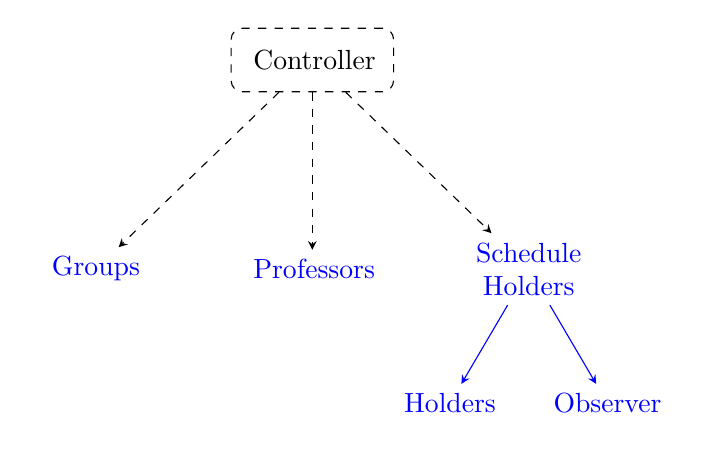
\begin{tikzpicture}[every node/.style={text width=1.5cm, align=center}]
    \node[draw, rounded corners,dashed, inner sep=8pt] (C) {Controller};
    \node[color=blue, below=2cm of C] (P) {Professors};
    \node[color=blue, left=of P]  (G) {Groups};
    \node[color=blue, right=of P] (H) {Schedule Holders};
    \draw[->, >=stealth, dashed] (C) -- (G);
    \draw[->, >=stealth, dashed] (C) -- (P);
    \draw[->, >=stealth, dashed] (C) -- (H);
    \node[color=blue, below=of H, xshift=-1cm] (HH) {Holders};
    \node[color=blue, below=of H, xshift=1cm]  (HO) {Observer};
    \draw[->, >=stealth, blue] (H) -- (HH);
    \draw[->, >=stealth, blue] (H) -- (HO);
  \end{tikzpicture}
  \end{center}

  \bigskip

  \blue{Groups} and \blue{Observer} have \underline{active} behaviour, while \\
  \blue{Professors} and \blue{Holders} exhibit only the \underline{reactive} one.

\end{frame}

% % % % % % % % % % % % % % % % % % % % % % % % % % % % % % % % % % % % % %

% % % % % % % % % % % % % % % % % % % %
\subsection{Group}


% % % % % % % % % % % % % % % % % % % % Candidates Creation

\againframe{candidate-def}

\begin{frame}{Group: Candidates Creation}
  \centering
  Each class consists of \emph{class-core} and \emph{instance} assignations

  \bigskip \bigskip

  \begin{block}{Class-Cores Pool}
    is a lazy random sequence of class-cores,
    that contain \underline{a class for each discipline}, needed by the group.

    \medskip

    \begin{enumerate}
      \item For each discipline needed select professors, that can teach it.
            Randomize professors lists.
      \item Lazily generate all possible combinations \emph{professor} -- \emph{discipline}.
      \item When getting next combination, assign the generating \emph{group}.
    \end{enumerate}
  \end{block}
\end{frame}

\begin{frame}{Group: Candidates Creation}
  \begin{block}{Day -- Time -- Room}
    \begin{enumerate}
      \item Generate random \emph{day}.
      \item Select random \emph{classroom}.
      \item Generate \emph{beginning time}.
      \item Get class duration from the \emph{discipline}, contained in argument class-core.
            Calculate \emph{end time}.
      \item Test \emph{end time} consistency (upper bound).
      \item Test \emph{time consistency} of the values from (1-4) using the history.
      \item If new values are consistent, add them to history, assign to class-core
            and return it.
            Otherwise, repeat from (1).
    \end{enumerate}
    Assignation for classes of same possible candidate is done with same
      history.
  \end{block}
\end{frame}


% % % % % % % % % % % % % % % % % % % % Action Part I

\begin{frame}{Group Action}
  \marginbox{-30pt 0 0 0}{
    \clipbox{-65pt 350 20 0}{ %{left bottom right top}
      \resizebox{\textwidth}{!}{
        \input{\rootdir/img/SolutionProcess-content.tikz}
      }
    }
  }
\end{frame}

% % % % % % % % % % % % % % % % % % % % Placement Intention

\begin{frame}{Group: Candidate Placement}
  If candidate was found coherent, try to put it in the \emph{common schedule}:
  \begin{itemize}
    \item \underline{Success} --- the agent ``goes to \green{sleep}'', until disturbed
    \item \underline{Conflicts} --- try \alert{win competence} or change candidate
  \end{itemize}
  \begin{block}{Conflicts}
    happen with candidates, already existing in current schedule
  \end{block}
  \centering
  \marginbox{-30pt 0 0 0}{
    \resizeinput[.5]{\rootdir/img/ConnectionMatrix/Conflict-content.tikz}
  }
\end{frame}

% % % % % % % % % % % % % % % % % % % % Action Part II

\begin{frame}{Group Action}
  \marginbox{-30pt 0 0 0}{
    \clipbox{-65pt 0 20 180}{ %{left bottom right top}
      \resizebox{\textwidth}{!}{
        \input{\rootdir/img/SolutionProcess-content.tikz}
      }
    }
  }
\end{frame}

% % % % % % % % % % % % % % % % % % % % Conflicts Resolution

\begin{frame}{Conflicts Resolution}
  A conflict arises \underline{between groups}.
  \\\medskip
  The ``newcomer'' candidate must have better quality than \underline{any}
  conflicting one.
  \\\bigskip
  \begin{block}{Quality Comparison}
    \centering \bigskip
    Ext. coherence $<$ Deep ext. coherence $<$ Disciplines priority
  \end{block}
  \medskip
  \begin{block}{External Coherence Comparison}
    \centering \bigskip
    Preliminary mode $<$ Final mode
  \end{block}
\end{frame}

% % % % % % % % % % % % % % % % % % % % Deep Coherence Assessment
\subsubsection{Deep External Coherence}

\begin{frame}{Deep External Coherence}
  \begin{columns}
    \begin{column}{.8\textwidth}
      \begin{itemize}
        \item[Depth 0:] internal coherence of the professors,
                  mentioned by candidate $\tilde{c}_i$ are accumulated.
        \item[Depth 1:] internal coherence of the group agents,
                  that have created candidates, mentioning groups from depth 0.
        \item[$\vdots$]
        \item[Even depth $j$:] internal coherence of the professors,
                  mentioned by candidates of the professors from depth $j-1$.
        \item[Depth $j+1$:] internal coherence of the groups,
                  that created candidates, mentioning of the professors from depth $j$.
        \item[$\vdots$]
        \item[Depth $N+1$:] Stop criterion.
                  All ``new'' coherence values were already retrieved at some previous depth.
      \end{itemize}
    \end{column}
  \end{columns}
\end{frame}


\input{\rootdir/img/ConnectionMatrix.tikz}

\newcommand*{\drawMatrix}[2][]{
  \def\d{#2}
  \connectionsMatrix[
      % row 5/.style={nodes={text=\Green}},
      row 6/.style={nodes={text=red}},
      #1]{m\d};
  \node[draw, color=blue, circle, thick, inner sep=5pt] at (m\d-5-1) {};
  \fith[dashed]{m\d}{6}{red}
  \usedh{m\d}{6}{red}
}

% \newcommand{\cohs}{}

\newcommand*{\showExtCoh}[5][]{
  \def\m{#2}
  \def\a{#3}
  \def\d{#4}
  \def\pss{#5}

  \gdef\cohs{}
  \gdef\first{1}
  \foreach \ps in \pss
    { \ifthenelse{\first=1}
          {\numgdef\first{0}}
          {\xappto\cohs{\noexpand\\[-4pt]}}
      \foreach \x in \ps {\xappto\cohs{, coh[\x]}}
     }
  \node[below=1em of \m, text width=9cm, align=center, #1]
      {External coherence of depth \d\ by $\a$:
       \begin{gather*}
         \Gamma\big( coh[\a] \cohs \big)
       \end{gather*}
       };
}

% col-color/.style args = {#1=#2}{column #1/.style={nodes={text=#2}}},
% row-color/.style args = {#1=#2}{row #1/.style={nodes={text=#2}}}


\begin{frame}{Deep External Coherence}
  \alert{No class} (or its references), \alert{belonging to conflicting candidate},
        can be used in the evaluation.
  \bigskip \bigskip
  \begin{columns}
    \begin{column}{.4\textwidth}
      \resizebox{\textwidth}{!}{
        \begin{tikzpicture}[
          col-color/.style args = {####1=####2}{column ####1/.style={nodes={text=####2}}},
          row-color/.style args = {####1=####2}{row ####1/.style={nodes={text=####2}}}
          ]
          \drawMatrix[col-color/.list={2=blue,4=blue,5=blue},
                      row-color/.list={5=blue}]{0};
          \fith{m0}{5}{blue}
          \fitv[dashed]{m0}{2}{blue}
          \fitv[dashed]{m0}{4}{blue}
          \fitv[dashed]{m0}{5}{blue}
          \showExtCoh{m0}{g_i}{0}{{p_1, p_*, p_k}}
        \end{tikzpicture}
        }
    \end{column}
    \begin{column}{.4\textwidth}
      \resizebox{\textwidth}{!}{
        \begin{tikzpicture}[
          col-color/.style args = {####1=####2}{column ####1/.style={nodes={text=####2}}},
          row-color/.style args = {####1=####2}{row ####1/.style={nodes={text=####2}}}
          ]
          \drawMatrix[right=2cm of m0,
                      col-color/.list={2=blue,4=blue,5=blue},
                      row-color/.list={5=blue,3=blue,7=blue}]{1};
          \fith[dotted]{m1}{5}{blue}
          \fitv{m1}{2}{blue}
          \fitv{m1}{4}{blue}
          \fitv{m1}{5}{blue}
          \fith[dashed]{m1}{3}{blue}
          \fith[dashed]{m1}{7}{blue}
          \showExtCoh{m1}{g_i}{1}{{p_1, p_*, p_k, g_2, g_n}}
        \end{tikzpicture}
      }
    \end{column}
  \end{columns}
\end{frame}

\begin{frame}{Deep External Coherence}
  \begin{columns}
    \begin{column}{.4\textwidth}
      \resizebox{\textwidth}{!}{
        \begin{tikzpicture}[
          col-color/.style args = {####1=####2}{column ####1/.style={nodes={text=####2}}},
          row-color/.style args = {####1=####2}{row ####1/.style={nodes={text=####2}}}
          ]
          \drawMatrix[below=2cm of m0,
                      col-color/.list={2=blue,4=blue,5=blue,6=blue,7=blue,8=blue},
                      row-color/.list={5=blue,3=blue,7=blue}]{2};
          \fith[dotted]{m2}{5}{blue}
          \fitv[dotted]{m2}{2}{blue}
          \fitv[dotted]{m2}{4}{blue}
          \fitv[dotted]{m2}{5}{blue}
          \fith{m2}{3}{blue}
          \fith{m2}{7}{blue}
          \fitv[dashed]{m2}{6}{blue}
          \fitv[dashed]{m2}{7}{blue}
          \fitv[dashed]{m2}{8}{blue}
          \showExtCoh{m2}{g_i}{2}{{p_1, p_*, p_k, g_2, g_n}, {p_*, p_*, p_m}}
        \end{tikzpicture}
      }
    \end{column}
    \begin{column}{.4\textwidth}
      \resizebox{\textwidth}{!}{
        \begin{tikzpicture}[
          col-color/.style args = {####1=####2}{column ####1/.style={nodes={text=####2}}},
          row-color/.style args = {####1=####2}{row ####1/.style={nodes={text=####2}}}
          ]
          \drawMatrix[below=2cm of m1,
                      col-color/.list={2=blue,4=blue,5=blue,6=blue,7=blue,8=blue},
                      row-color/.list={5=blue,3=blue,7=blue,2=blue,4=blue}]{3};
          \fith[dotted]{m3}{5}{blue}
          \fitv[dotted]{m3}{2}{blue}
          \fitv[dotted]{m3}{4}{blue}
          \fitv[dotted]{m3}{5}{blue}
          \fith[dotted]{m3}{3}{blue}
          \fith[dotted]{m3}{7}{blue}
          \fitv{m3}{6}{blue}
          \fitv{m3}{7}{blue}
          \fitv{m3}{8}{blue}
          \fith[dashed]{m3}{2}{blue}
          \fith[dashed]{m3}{4}{blue}
          \showExtCoh{m3}{g_i}{3}{{p_1, p_*, p_k, g_2, g_n}, {p_*, p_*, p_m, g_1, g_*}}
        \end{tikzpicture}
      }
    \end{column}
  \end{columns}
\end{frame}

\begin{frame}{Deep External Coherence}
  \begin{columns}
    \begin{column}{.6\textwidth}
      \resizebox{\textwidth}{!}{
        \begin{tikzpicture}[
          col-color/.style args = {####1=####2}{column ####1/.style={nodes={text=####2}}},
          row-color/.style args = {####1=####2}{row ####1/.style={nodes={text=####2}}}
          ]
          \drawMatrix[below=2cm of m2,
                      col-color/.list={2=blue,4=blue,5=blue,6=blue,7=blue,8=blue,3=blue},
                      row-color/.list={5=blue,3=blue,7=blue,2=blue,4=blue}]{4};
          \fith[dotted]{m4}{5}{blue}
          \fitv[dotted]{m4}{2}{blue}
          \fitv[dotted]{m4}{4}{blue}
          \fitv[dotted]{m4}{5}{blue}
          \fith[dotted]{m4}{3}{blue}
          \fith[dotted]{m4}{7}{blue}
          \fitv[dotted]{m4}{6}{blue}
          \fitv[dotted]{m4}{7}{blue}
          \fitv[dotted]{m4}{8}{blue}
          \fith{m4}{2}{blue}
          \fith{m4}{4}{blue}
          \fitv[dashed]{m4}{3}{blue}
          \showExtCoh{m4}{g_i}{4 (max)}
            {{p_1, p_*, p_k, g_2, g_n}, {p_*, p_*, p_m, g_1, g_*, p_2}}
        \end{tikzpicture}
      }
    \end{column}
    \begin{column}{.4\textwidth}
      \begin{block}{Common Goal $\Gamma$}
        combines coherence, making no difference between value origins
      \end{block}
      \begin{examples}
        \begin{itemize}
          \item \emph{arithmetic} mean $\frac{\sum_n}{n}$ \emph{mean}.
          \item \emph{geometric}  mean $\sqrt[\leftroot{-2}\uproot{2}n]{\prod_n}$
          \item $\dots$
        \end{itemize}
      \end{examples}
    \end{column}
  \end{columns}

\end{frame}

% % % % % % % % % % % % % % % % % % % % Disciplines Priority
\subsubsection{Disciplines Priority}

\begin{frame}{Disciplines Priority}{Candidate ``Rarity''}
  \begin{block}{Discipline ``Rarity'' / Priority}
    \begin{columns}
      \begin{column}{-.5cm}\end{column}
      \begin{column}{.65\textwidth}\\
        is ratio
        \begin{itemize}
          \item[of] groups enrolled to the discipline ($N_G$)
          \item[to] professors able to teach it ($N_P$).
        \end{itemize}
      \end{column}
      \begin{column}{.1\textwidth}
        $$\rho^d = \dfrac{N_G}{N_P}$$
      \end{column}
      \begin{column}{.1\textwidth}\end{column}
    \end{columns}
    \bigskip
    Discipline $d$ is considered \alert{``rare''} if its priority
    $\rho_d$ is higher than some threshold
  \end{block}
  \begin{block}{Candidate ``Rarity''}
    \begin{columns}
      \begin{column}{.4\textwidth}
        \bigskip
        $$\rho_{\tilde{c}} = \sum\limits_{d \in D'_{\tilde{c}}}
                \rho^d \cdot \mathsmaller{ \sum\limits_{c \in \tilde{c}'_d}
                                     \mathit{duration}\, c }$$
      \end{column}
      \begin{column}{.4\textwidth}
        \begin{align*}
          D'_{\tilde{c}} &= \lbrace d ~|~ d ~\mathit{referenced\,by}~ \tilde{c};~
                                        \rho_d > \rho_* \rbrace\\
          \tilde{c}'_d &= \lbrace c ~|~ c \in \tilde{c};~ c ~\mathit{is\,class\,for}~ d \rbrace
        \end{align*}
      \end{column}
    \end{columns}
  \end{block}
\end{frame}


% % % % % % % % % % % % % % % % % % % % % % % % % % % % % % % % % % % % % %

% % % % % % % % % % % % % % % % % % % % % % % % % % % % % % % % % % % % % % % %


% % % % % % % % % % % % % % % % % % % % % % % % % % % % % % % % % % % % % % VII
\section{Results}
% % % % % % % % % % % % % % % % % % % % Data
\subsection{Data}

\begin{frame}{Data Definition}
  \begin{mdframed}[leftmargin=1cm, hidealllines=true]
    \begin{itemize}
      \item[\underline{Institution:}]
        \begin{itemize}
          \item Static:
                \begin{enumerate}
                  \item[a.] \emph{timetable},
                  \item[b.] \emph{disciplines},
                  \item[c.] \emph{classrooms}.
                \end{enumerate}
          \item Participants --- for each \underline{group} and \underline{professor}:\\
                \begin{enumerate}
                  \item \emph{unique name},
                  \item \emph{can teach} / \emph{need} disciplines
                  \item \emph{obligations}
                \end{enumerate}
        \end{itemize}
      \item[\underline{Personal:}]
        \begin{itemize}
          \item[] for each \underline{group} and \underline{professor}:
          \begin{enumerate}
            \item[4.] \emph{preferences}
          \end{enumerate}
        \end{itemize}
    \end{itemize}
  \end{mdframed}
\end{frame}

% % % % % % % % % % % % % % % % % % % %
\subsubsection{Static Data}

\begin{frame}{Test Data: Disciplines}
  \centering
  \resizeinput[.7]{\rootdir/TestResults/TestData/Disciplines}
\end{frame}

\begin{frame}{Test Data: Classrooms}
  \begin{columns}
    \begin{column}{.5\textwidth}
      \resizeinput[.8]{\rootdir/TestResults/TestData/Classrooms}
    \end{column}
    \begin{column}{.4\textwidth}
      \resizeinput{\rootdir/TestResults/TestData/Requirements}
    \end{column}
  \end{columns}
\end{frame}

\begin{frame}{Test Data: Groups}{Part 1}
  \resizeinput{\rootdir/TestResults/TestData/Groups-Static}
\end{frame}

\begin{frame}{Test Data: Professors}{Part 1}
  \centering
  \resizeinput[.65]{\rootdir/TestResults/TestData/Professors-Static}
\end{frame}

% % % % % % % % % % % % % % % % % % % %
\subsubsection{Personal Data}

\begin{frame}{Test Data: Groups \& Professors}{Part 2}
  \begin{columns}[t]
    \begin{column}{.5\textwidth}
      \resizeinput{\rootdir/TestResults/TestData/Groups-Personal}
    \end{column}
    \begin{column}{.5\textwidth}
      \resizeinput{\rootdir/TestResults/TestData/Professors-Personal}
    \end{column}
  \end{columns}
\end{frame}

% % % % % % % % % % % % % % % % % % % % Results
\subsection{Results}


% % % % % % % % % % % % % % % % % % % % % % % % % % % % % % % % % % % % % % VIII
\section{Improvements}
\subsection{Students Representation}
\subsection{Classrooms Representation}
\subsection{Roles Extension}


\end{document}
